\documentclass[pdf,16pt]{beamer}
\mode<presentation>{\usetheme{Warsaw}}
\usepackage{fontspec}   %加這個就可以設定字體
\usepackage{xeCJK}       %讓中英文字體分開設置

%
\usepackage{listings}
\usepackage{graphicx} % Allows including images
\usepackage{booktabs} % Allows the use of \toprule, \midrule and \bottomrule in tables
\setCJKmainfont{LiHei Pro} %設定中文為系統上的字型,而英文不去更動,使用原TeX字型
\XeTeXlinebreaklocale "zh"             %這兩行一定要加,中文才能自動換行
\XeTeXlinebreakskip = 0pt plus 1pt     %這兩行一定要加,中文才能自動換行

%% preamble
\title{Git \& Github}
\author{曹又霖}

\defbeamertemplate{footline}{centered page number}
{%
  \hspace*{\fill}%
  \usebeamercolor[fg]{page number in head/foot}%
  \usebeamerfont{page number in head/foot}%
  \insertpagenumber%
  \hspace*{\fill}\vskip2pt%
}

\setbeamertemplate{footline}[centered page number]
\setbeamertemplate{caption}[numbered]

\begin{document}

  %% title frame
  \begin{frame}
    \titlepage
  \end{frame}
  
  \begin{frame}
    \frametitle{大綱} % Table of contents slide, comment this block out to remove it
    \tableofcontents % Throughout your presentation, if you choose to use \section{} and \subsection{} commands, these will automatically be printed on this slide as an overview of your presentation
  \end{frame}
  
  \begin{section}{版本控制}
    \begin{subsection}{簡介}
      %% normal frame
      \begin{frame}{為什麼要版本控制}
        \begin{itemize}
          \item 改錯程式或誤刪檔案
          \item 還原之前寫的版本
          \item 團隊合作開發
          \item 軟體發行時,要分成穩定版和開發版
        \end{itemize}
      \end{frame}
    \end{subsection}
    
    \begin{subsection}{版本控制總類}
      \begin{frame}{本地端版本控制}
        \begin{figure}[h!]
          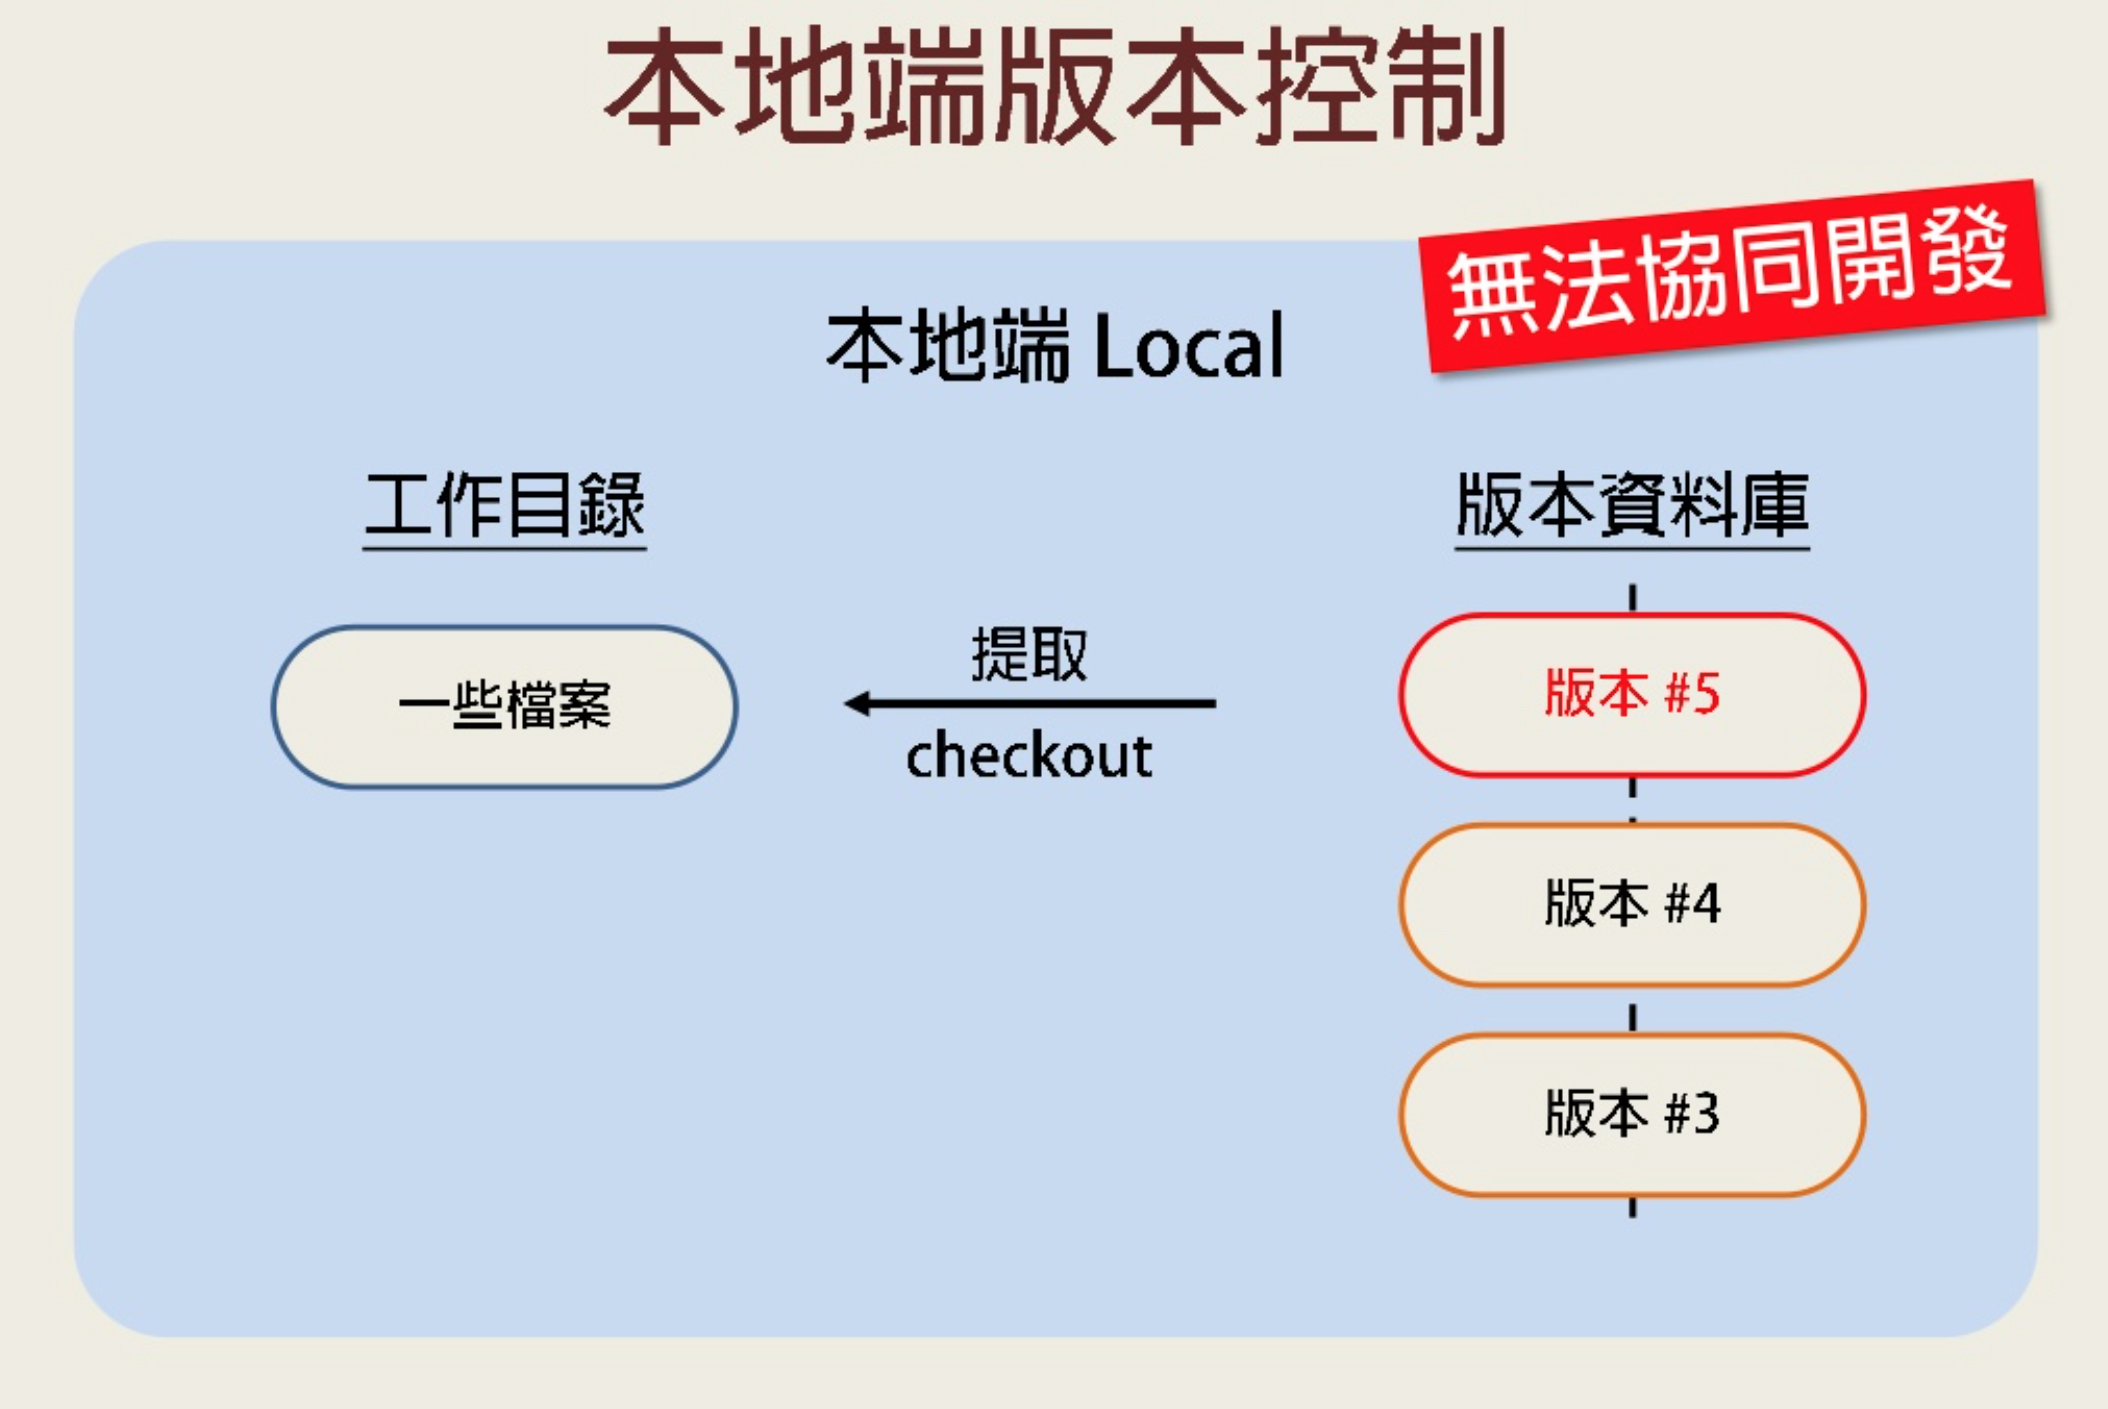
\includegraphics[width=0.8\textwidth]{images/001.jpg} 
          \caption{本地端版本控制}
        \end{figure}
      \end{frame}
      
      \begin{frame}{中心式版本控制}
        \begin{figure}[h!]
          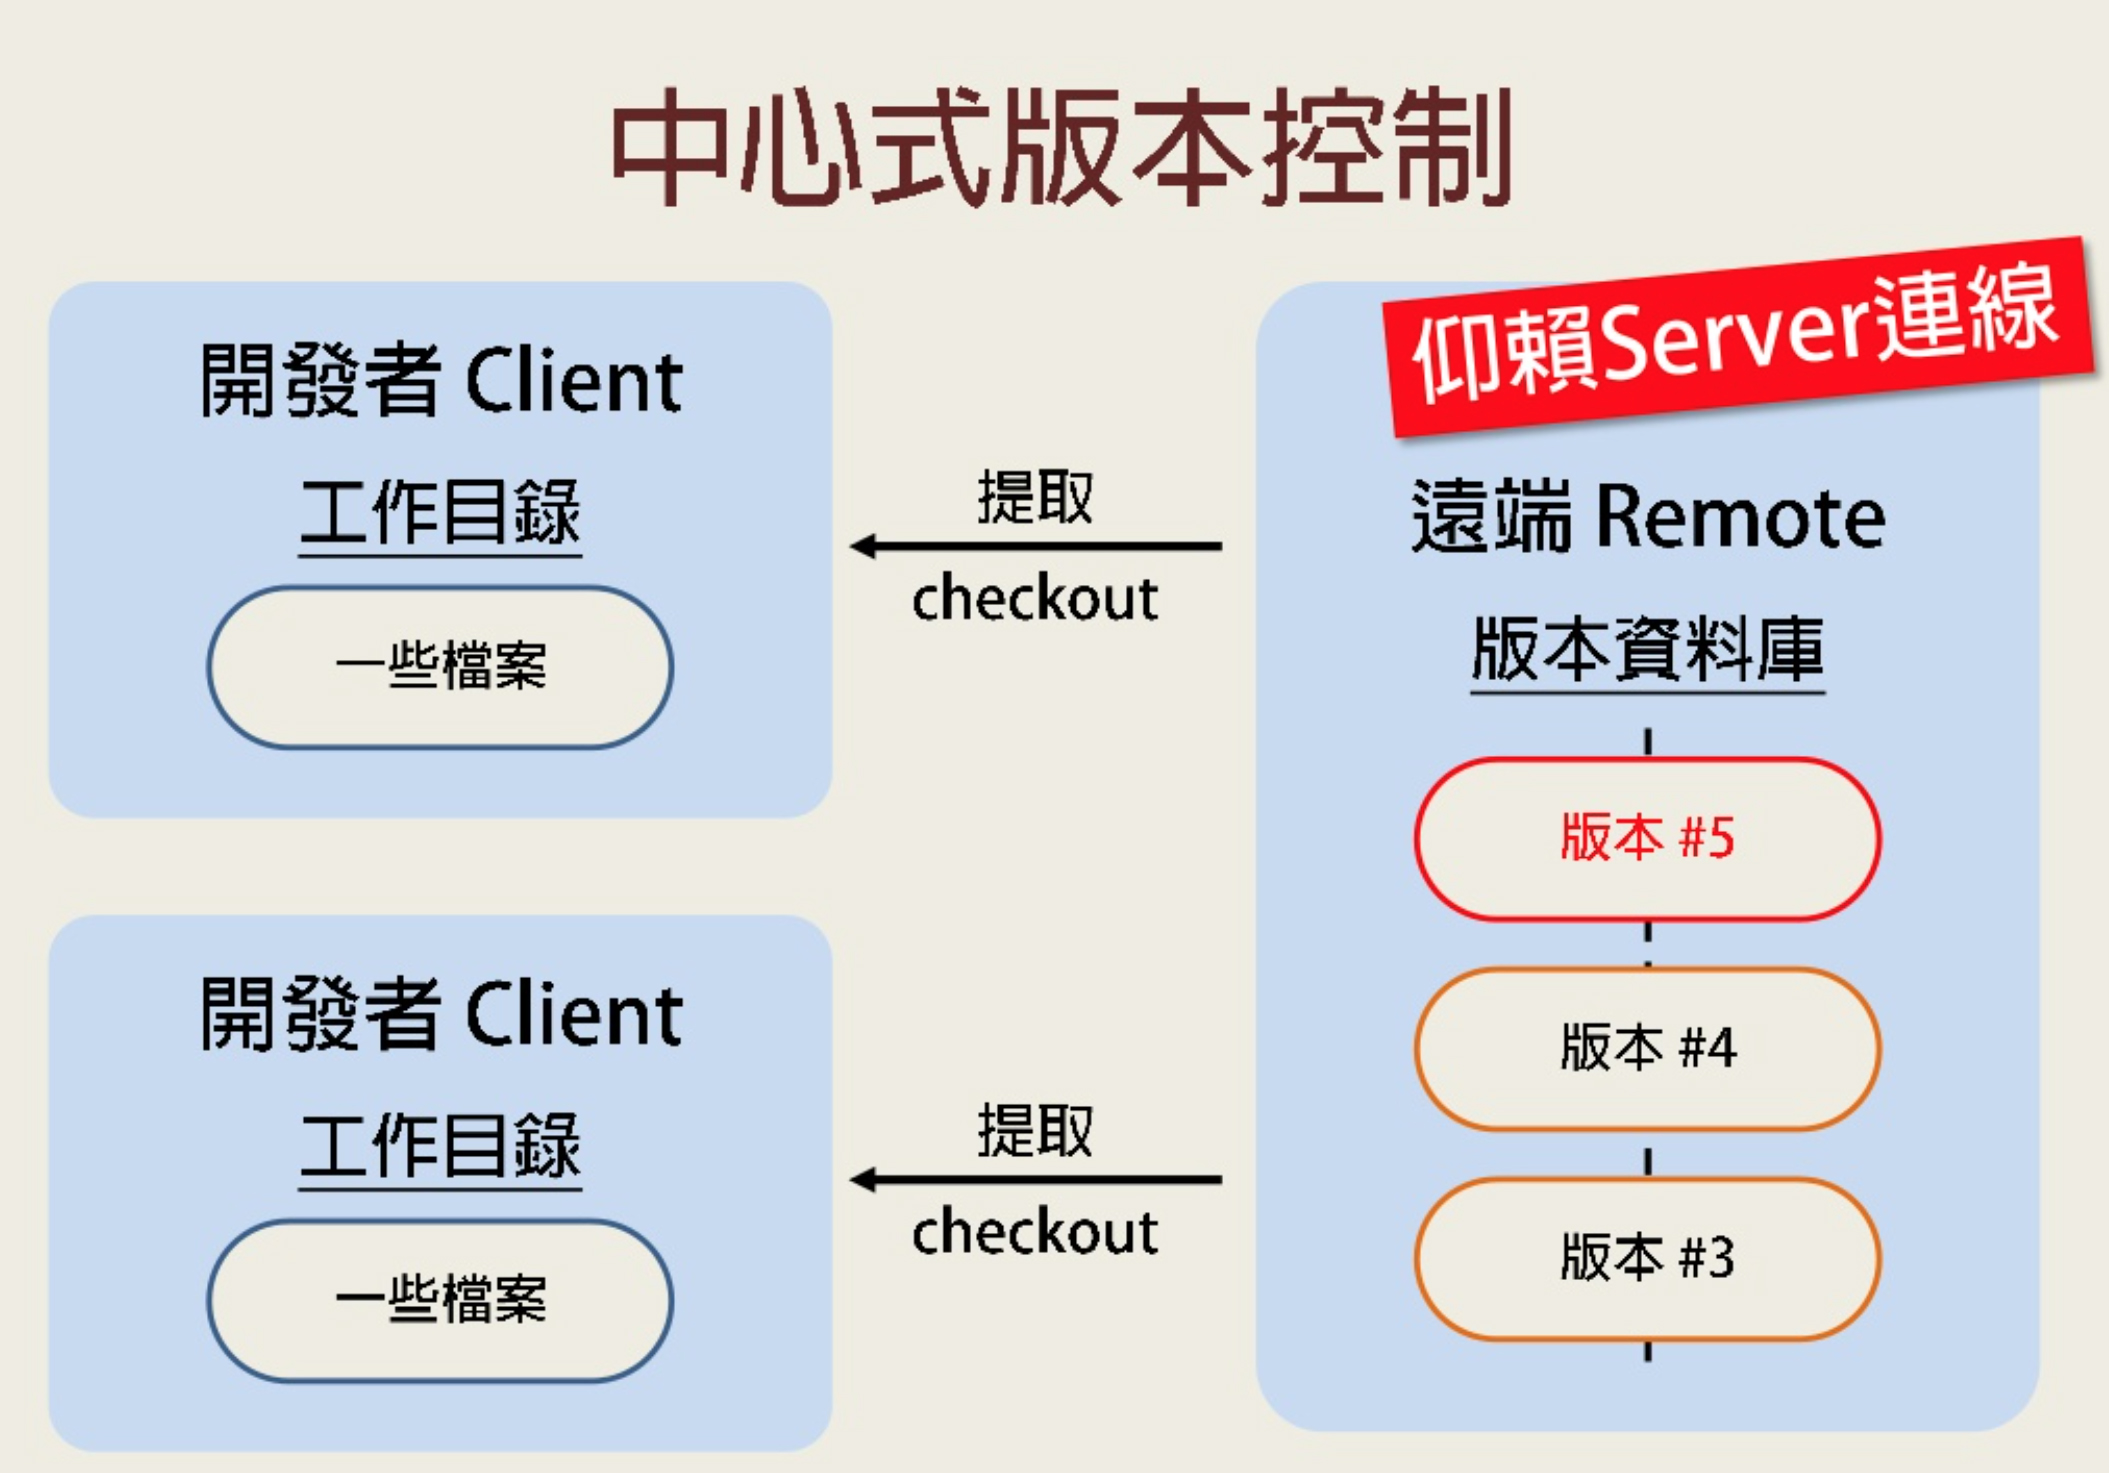
\includegraphics[width=0.8\textwidth]{images/002.jpg} 
          \caption{中心式版本控制}
        \end{figure}
      \end{frame}
      
      \begin{frame}{分散式版本控制}
        \begin{figure}[h!]
          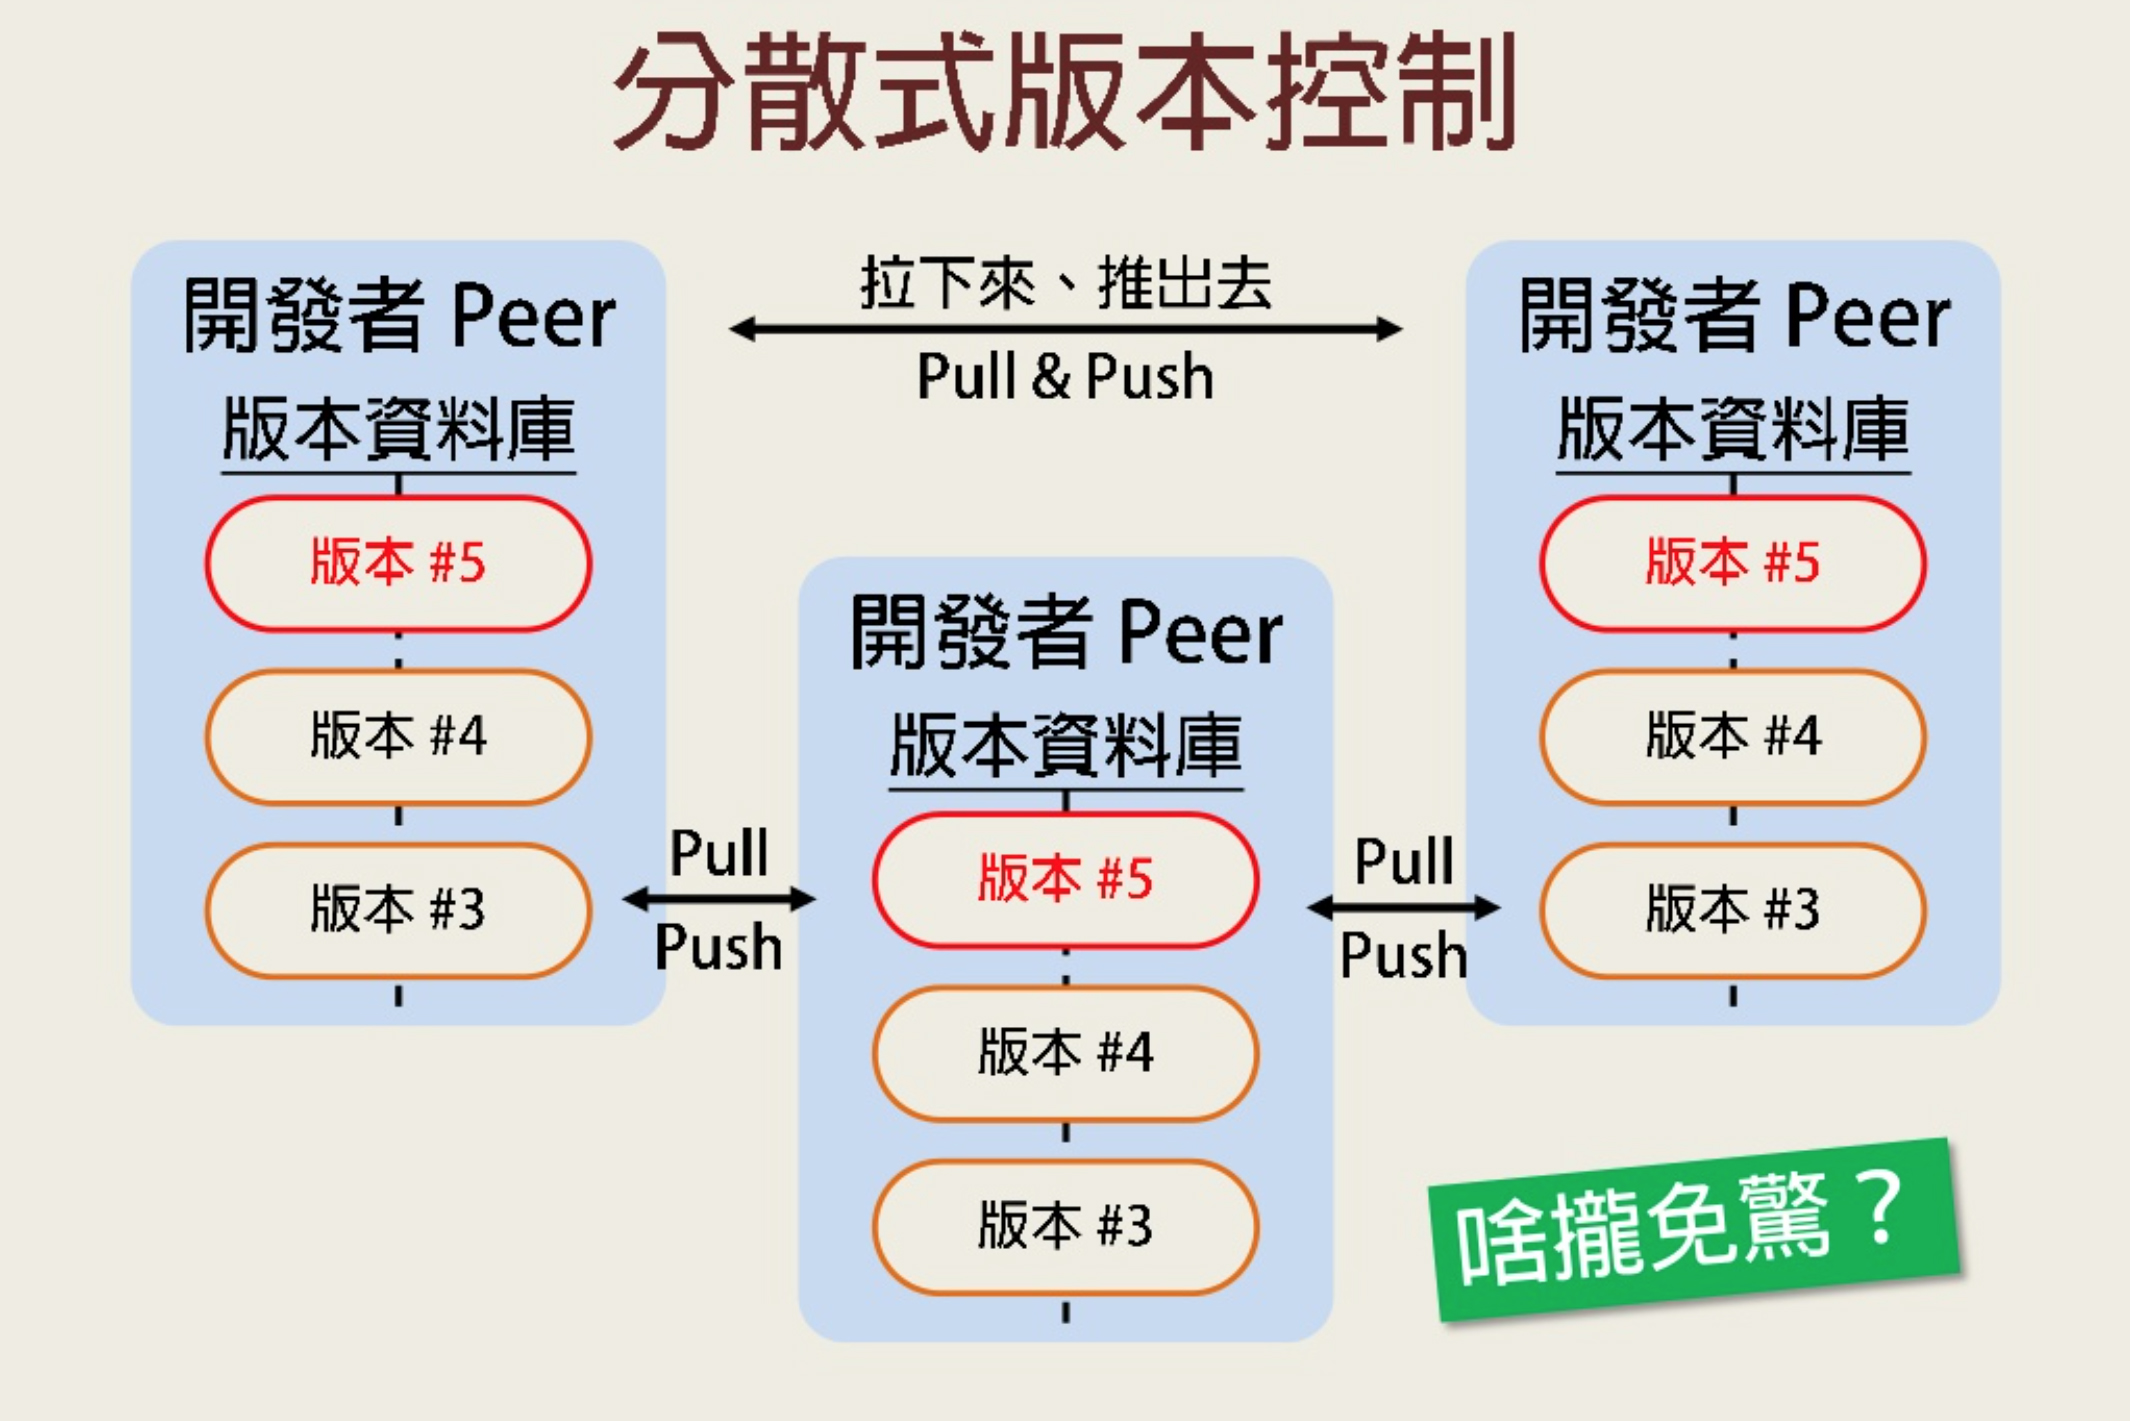
\includegraphics[width=0.8\textwidth]{images/003.jpg} 
          \caption{分散式版本控制}
        \end{figure}
      \end{frame}
    \end{subsection}
  \end{section}

  \begin{section}{Git}
    \begin{subsection}{簡介}
      %% normal frame
      \begin{frame}{Git}
        \begin{itemize}
          \item 發明人 Linus Torvalds (即Linux創始人)
          \item 目的為管理Linux程式碼
          \item 是一分散式版本控制
        \end{itemize}
      \end{frame}
      
      \begin{frame}{Git目標}
        \begin{itemize}
          \item 速度快
          \item 簡單使用
          \item 非線性開發
          \item 分散式開發
        \end{itemize}
      \end{frame}
      
      \begin{frame}{安裝Git}
        \begin{itemize}
          \item 安裝Git
          \begin{itemize}
            \item \url{https://help.github.com/articles/set-up-git/}
          \end{itemize}
          \item 安裝Git GUI
          \begin{itemize}
            \item GitX (Mac OS X)
            \item TortoiseGit (Windows)
          \end{itemize}
        \end{itemize}
      \end{frame}
    \end{subsection}
    
    \begin{subsection}{使用教學}
      \begin{frame}{設定Git}
        \begin{block}{設定名稱}
          git config -\phantom{}-global user.name "Maplewing"
        \end{block}
        \begin{block}{設定Email}
          git config -\phantom{}-global user.email "sinmaplewing@gmail.com"
        \end{block}
      \end{frame}
      
      \begin{frame}{建立一個Git Repository}
        \begin{itemize}
          \item Repository(倉庫):版本控制系統的管轄之下的儲存位置。
          \item 有兩種方法可以建立Git Repo:
        \end{itemize}
        \begin{block}{創建新的Git Repo}
          git init
        \end{block}
        \begin{block}{複製一個現有的Git Repo}
          git clone \url{https://github.com/sinmaplewing/Mini_Monopoly.git}
        \end{block}
      \end{frame}
      
      \begin{frame}{加入檔案}
        \begin{figure}[h!]
          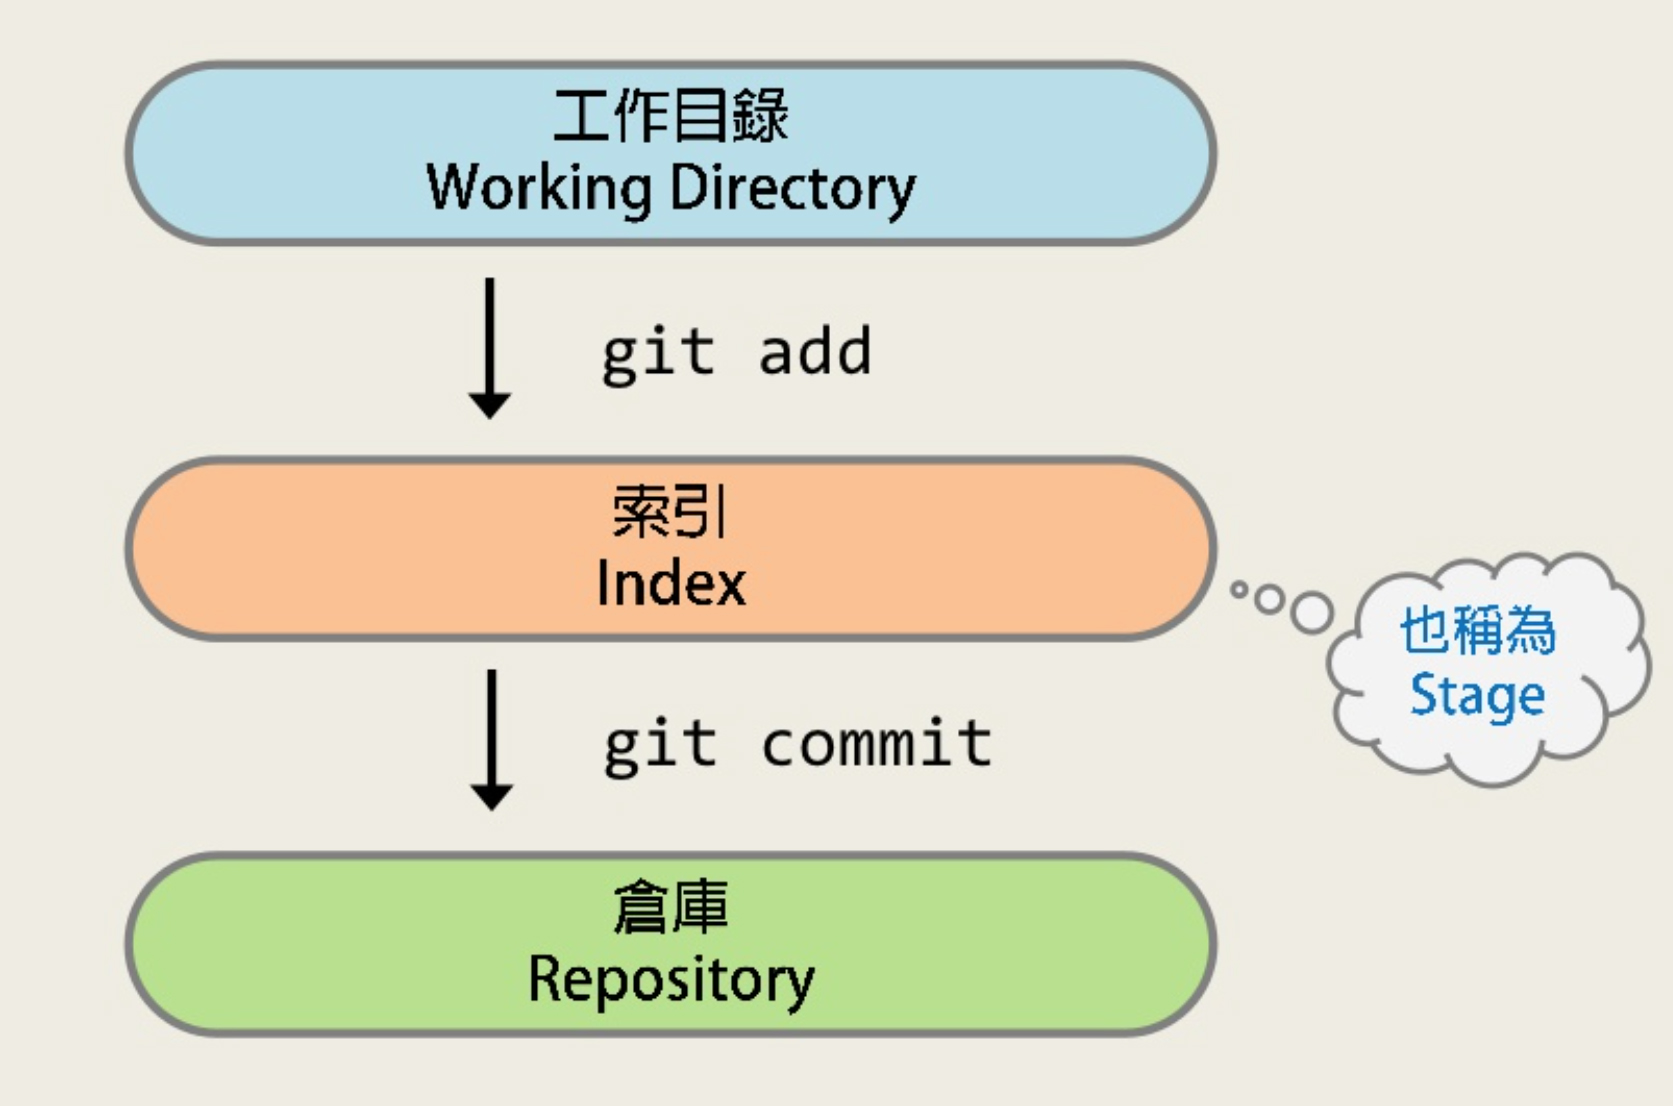
\includegraphics[width=0.8\textwidth]{images/004.jpg} 
          \caption{加入檔案流程}
        \end{figure}
      \end{frame}
      
      \begin{frame}{加入檔案}
        \begin{block}{加入檔案進入Stage}
          git add code.c\\
          git add .
        \end{block}
        \begin{block}{將變更記錄送入Repo}
          git commit -m "Add Code.c"\\
          git commit -a
        \end{block}
      \end{frame}
      
      \begin{frame}{檔案管理}
        \begin{itemize}
          \item Git會管理空檔案,但不理會空資料夾。
        \end{itemize}
        \begin{block}{改名檔案或是移動檔案}
          git mv code.c code.cpp
        \end{block}
        \begin{block}{刪除檔案}
          git rm code.c
        \end{block}
      \end{frame}
      
      \begin{frame}{.gitignore}
        \begin{itemize}
          \item 告訴Git哪些檔案不用加入。
          \item \url{https://github.com/github/gitignore}:這裡有大部分專案的.gitignore template可以參考。
        \end{itemize}
      \end{frame}
      
      \begin{frame}{狀態與紀錄}
        \begin{block}{觀看目前狀態}
          git status
        \end{block}
        \begin{block}{觀看commit紀錄}
          git log\\
          git log -\phantom{}-oneline\\
          git log -\phantom{}-oneline -\phantom{}-decorate -\phantom{}-graph
        \end{block}
        \begin{block}{觀看差別}
          git diff
        \end{block}
      \end{frame}
      
      \begin{frame}{復原檔案}
        \begin{block}{復原至上次commit的內容}
          git checkout HEAD\textasciicircum\\
          git checkout HEAD\textasciicircum\phantom{} code.c
        \end{block}
        \begin{block}{將檔案變回unstage狀態,不更動檔案}
          git reset HEAD code.c
        \end{block}
      \end{frame}
      
      \begin{frame}{使用分支}
        \begin{itemize}
          \item 預設分支為master
        \end{itemize}
        \begin{block}{查看目前分支}
          git branch
        \end{block}
        \begin{block}{創建新分支並移過去}
          git checkout -b newbranch
        \end{block}
        \begin{block}{移動分支}
          git checkout master
        \end{block}
        \begin{block}{合併指定分支到目前所在分支}
          git merge newbranch
        \end{block}
        
      \end{frame}
      
    \end{subsection}
   \end{section}
   
   \begin{section}{Github}
    \begin{subsection}{簡介}
      \begin{frame}{Github}
        \begin{figure}[h!]
          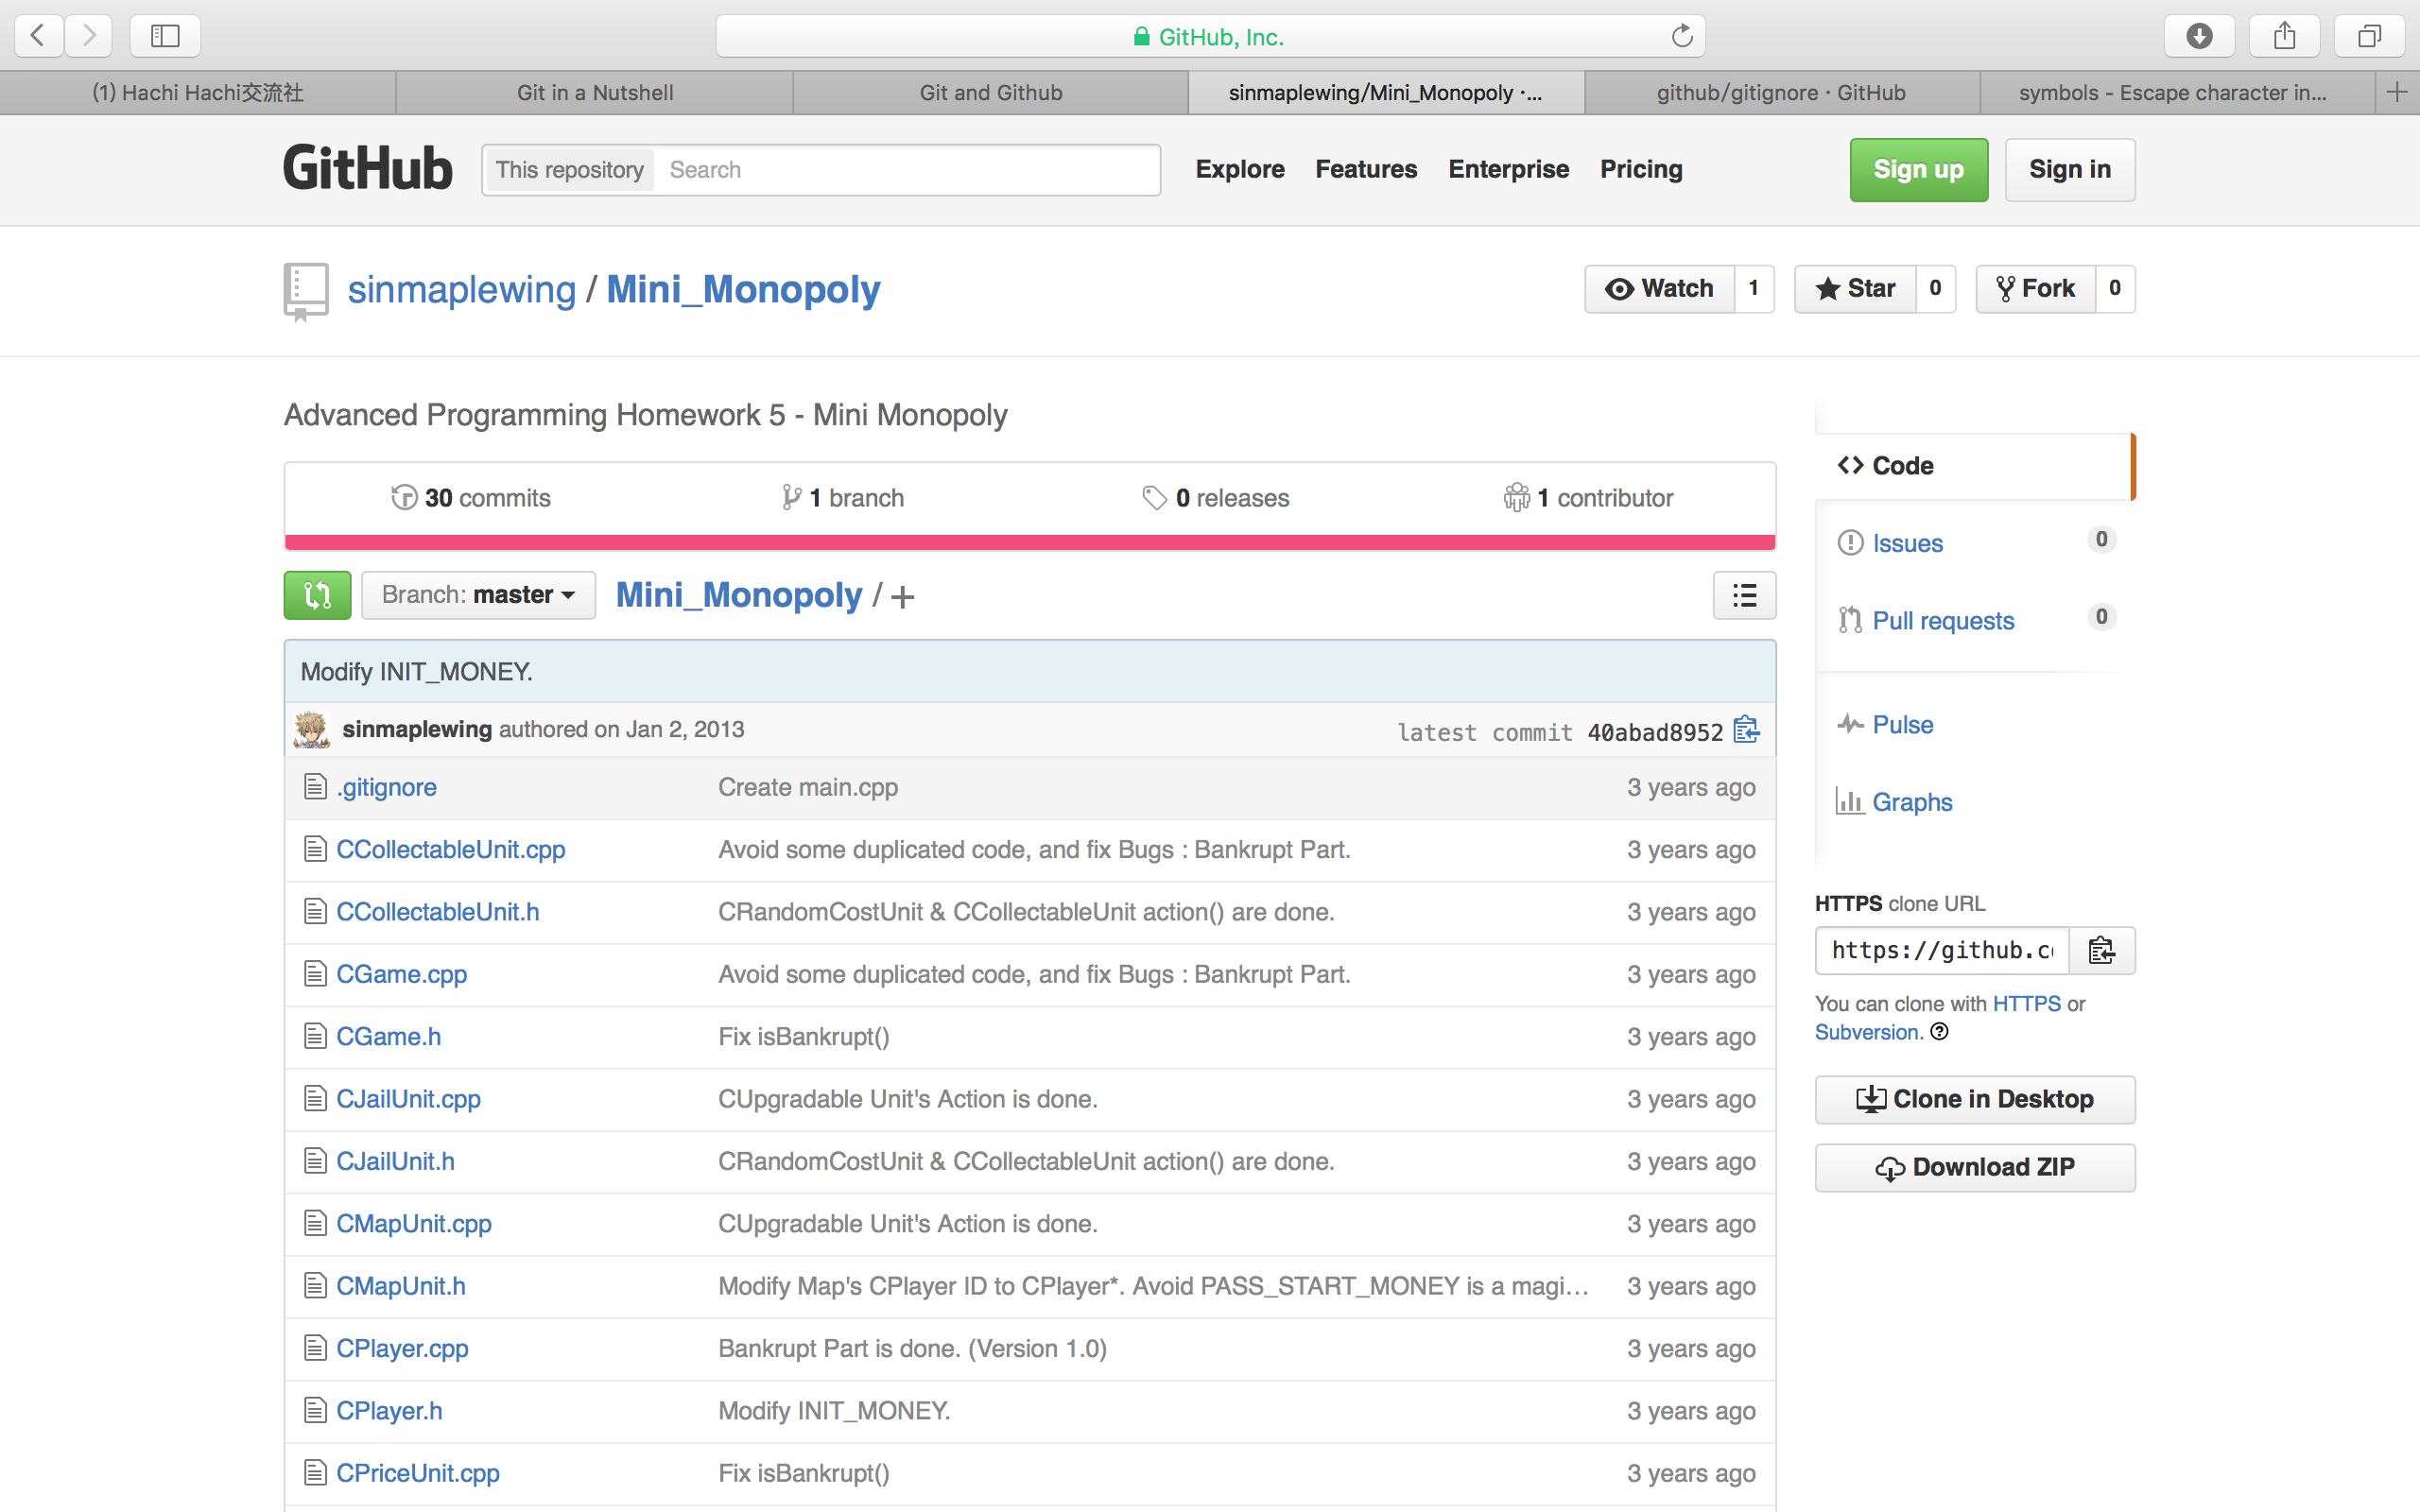
\includegraphics[width=0.8\textwidth]{images/005.png} 
          \caption{Github}
        \end{figure}
      \end{frame}
      
      \begin{frame}{Github}
        \begin{itemize}
          \item 線上的Repository
          \item 可創建Repo、fork Repo或是共同合作
        \end{itemize}
      \end{frame}
    \end{subsection}
    
    \begin{subsection}{使用說明}
      \begin{frame}{使用Github}
        \begin{block}{設定Remote}
          git remote add origin \url{Repo_url}
        \end{block}
        
        \begin{block}{將Local的變更推到Remote上}
          git push -u origin master
        \end{block}
        
        \begin{block}{將Remote的變更拉到Local上}
          git pull\\
          git pull origin master
        \end{block}
        
      \end{frame}
      
      \begin{frame}{Demo}
        Demo!
      \end{frame}
     
    \end{subsection}
    
   \end{section}
   
   \begin{section}{參考資料}
    \begin{subsection}{參考資料}
      \begin{frame}{參考資料}
        \begin{itemize}
          \item Git in a Nutshell: \url{http://www.slideshare.net/Dannvix/git-in-a-nutshell}
          \item Git \& Github: \url{http://www.slideshare.net/ihower/git-and-github-7306407}
          \item 連猴子都能懂的Git入門指南: \url{https://backlogtool.com/git-guide/tw/}
          \item Git 版本控制系統| ihower 的Git 教室: \url{https://ihower.tw/git/}
          \item Git 初學筆記 - 指令操作教學: \url{http://blog.longwin.com.tw/2009/05/git-learn-initial-command-2009/}
        \end{itemize}
      \end{frame}
     \end{subsection}
   \end{section}
\end{document}
